\paragraph{IUE03 Visualizar rutinas} \hspace{1cm}\\ 
\label{pant:IUE03}

\textbf{\textcolor[rgb]{0, 0, 0.545098}{Objetivo}}\\
Esta pantalla permite al Entrenador visualizar las listas de ejercicios de calentamiento, movimientos de técnica y rutinas de entrenamiento. Por cada rutina disponible se pueden modificar los identificadores o bien dar de baja.\\

\textbf{\textcolor[rgb]{0, 0, 0.545098}{Diseño}}\\
En la figura \ref{fig:IUE03} se muestra la pantalla \nameref{fig:IUE03}, la cual muestra al Entrenador tres elementos diferentes en los cuales se enlistan los ejercicios de calentamiento, movimientos de técnica y rutinas de entrenamiento registrados en la herramienta.\\

En la parte inferior izquierda se encuentran los botones de Agregar rutina y Regresar.

\begin{figure}[H]
	\centering
		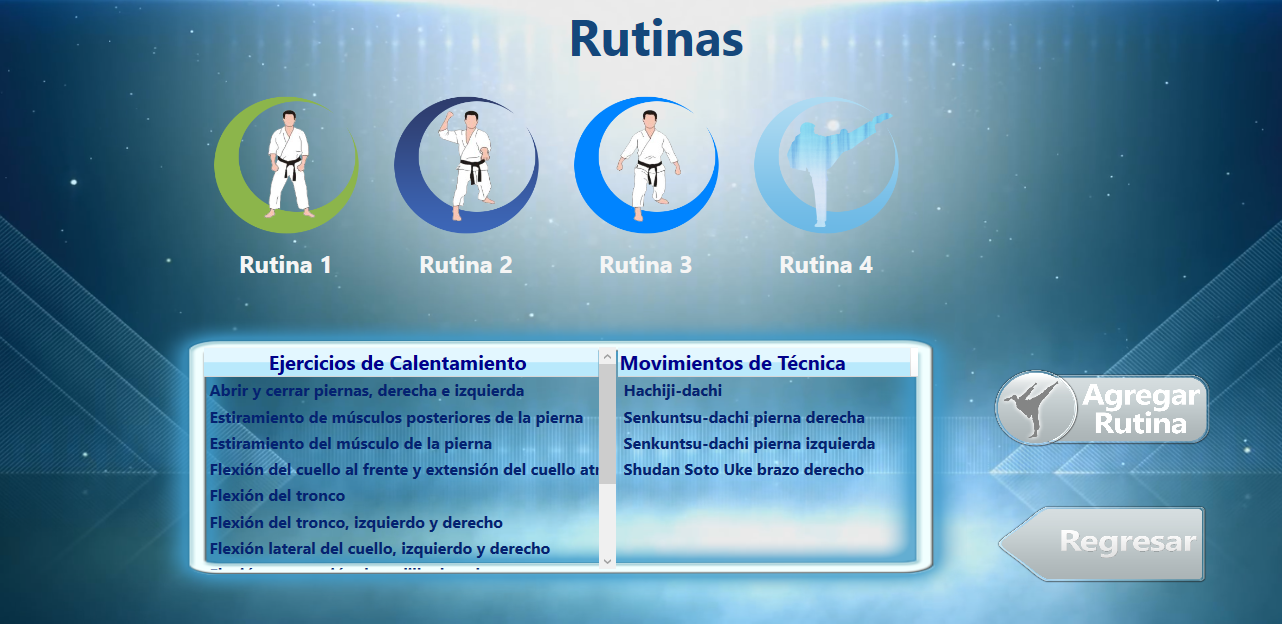
\includegraphics[scale=0.5]{./Figuras/Pantallas/IUE03Visualizar_rutinas}
	\caption{IUE03 Visualizar rutinas}
	\label{fig:IUE03}
\end{figure}

\textbf{\textcolor[rgb]{0, 0, 0.545098}{Controles}}
\begin{itemize}
	\item \textbf{\textcolor[rgb]{0, 0, 0.545098}{Rutinas de entrenamiento:}} Permite seleccionar al Entrenador alguna Rutina de entrenamiento. Una vez que se realice una selección, se muestra el menú \nameref{menu:ME03}.
\end{itemize}
\vspace{1em}

\textbf{\textcolor[rgb]{0, 0, 0.545098}{Comandos}}
\begin{itemize}
	\item \textbf{\textcolor[rgb]{0, 0, 0.545098}{Agregar rutina:}} Permite al Entrenador agregar una rutina por lo que hace una redirección a la pantalla \nameref{pant:IUE03.1}.
	\item \textbf{\textcolor[rgb]{0, 0, 0.545098}{Regresar:}} Muestra el menú principal \nameref{menu:ME01}.
\end{itemize}
\vspace{1em}

\textbf{\textcolor[rgb]{0, 0, 0.545098}{Mensajes}}\\
	
\textbf{\nameref{msj:MSG01}}: Se muestra en la pantalla \nameref{pant:IUE03}, cuando se realice una eliminación exitosa.\\

\textbf{\nameref{msj:MSG09}}: Se muestra en la pantalla \nameref{pant:IUE03} cuando el Entrenador desee eliminar una rutina que se encuentre asignada a un Practicante.\\
	
\textbf{\nameref{msj:MSG24}}: Se muestra en el menú principal \nameref{menu:ME01} cuando debido a un error de conexión no se muestren los elementos de forma correcta.\\

\clearpage